\chapter{Introducción}

\section{Motivación}
\label{sec:motivacion}

Este trabajo se realiza a partir de la necesidad de Valeo, una empresa del ámbito automobilístico, de realizar pruebas más especificas sobre los faros que producen. El laboratorio de GranaSAT, del que mi tutor forma parte, fue el encargado de desarrollar las primeras versiones del dispositivo, que fueron anteriormente presentadas como Trabajos de Fin de Grado por Luis Sánchez (autor de la PCB y todo el apartado electrónico) y Rubén Sánchez (desarrollador de una parte del firmware), respectivamente.

% TODO: Explicar aquí cómo es el dispositivo
% Este dispositivo está compuesto por un Arduino... con una pantalla... genera señales PWM... que son...

Este dispositivo está compuesto por un Arduino Mega 2560, una pantalla LCD de 4 líneas, un \textit{rotary encoder} y 8 conectores de salida. Por cada uno de estos 8 conectores se produce una salida PWM configurable por el usuario, pensada para conectar y probar los distintos modos del faro de un vehículo. En la \autoref{fig:pwmbox_top} incluída se puede ver la parte superior del dispositivo. Por otro lado, la \autoref{fig:pwmbox_side} muestra su lateral.

\begin{figure}
    \centering
    \includegraphics[width=\textwidth]{pwmbox_top.jpg}
    \caption{Dispositivo PWM Box desde arriba.}
    \label{fig:pwmbox_top}
\end{figure}

\begin{figure}
    \centering
    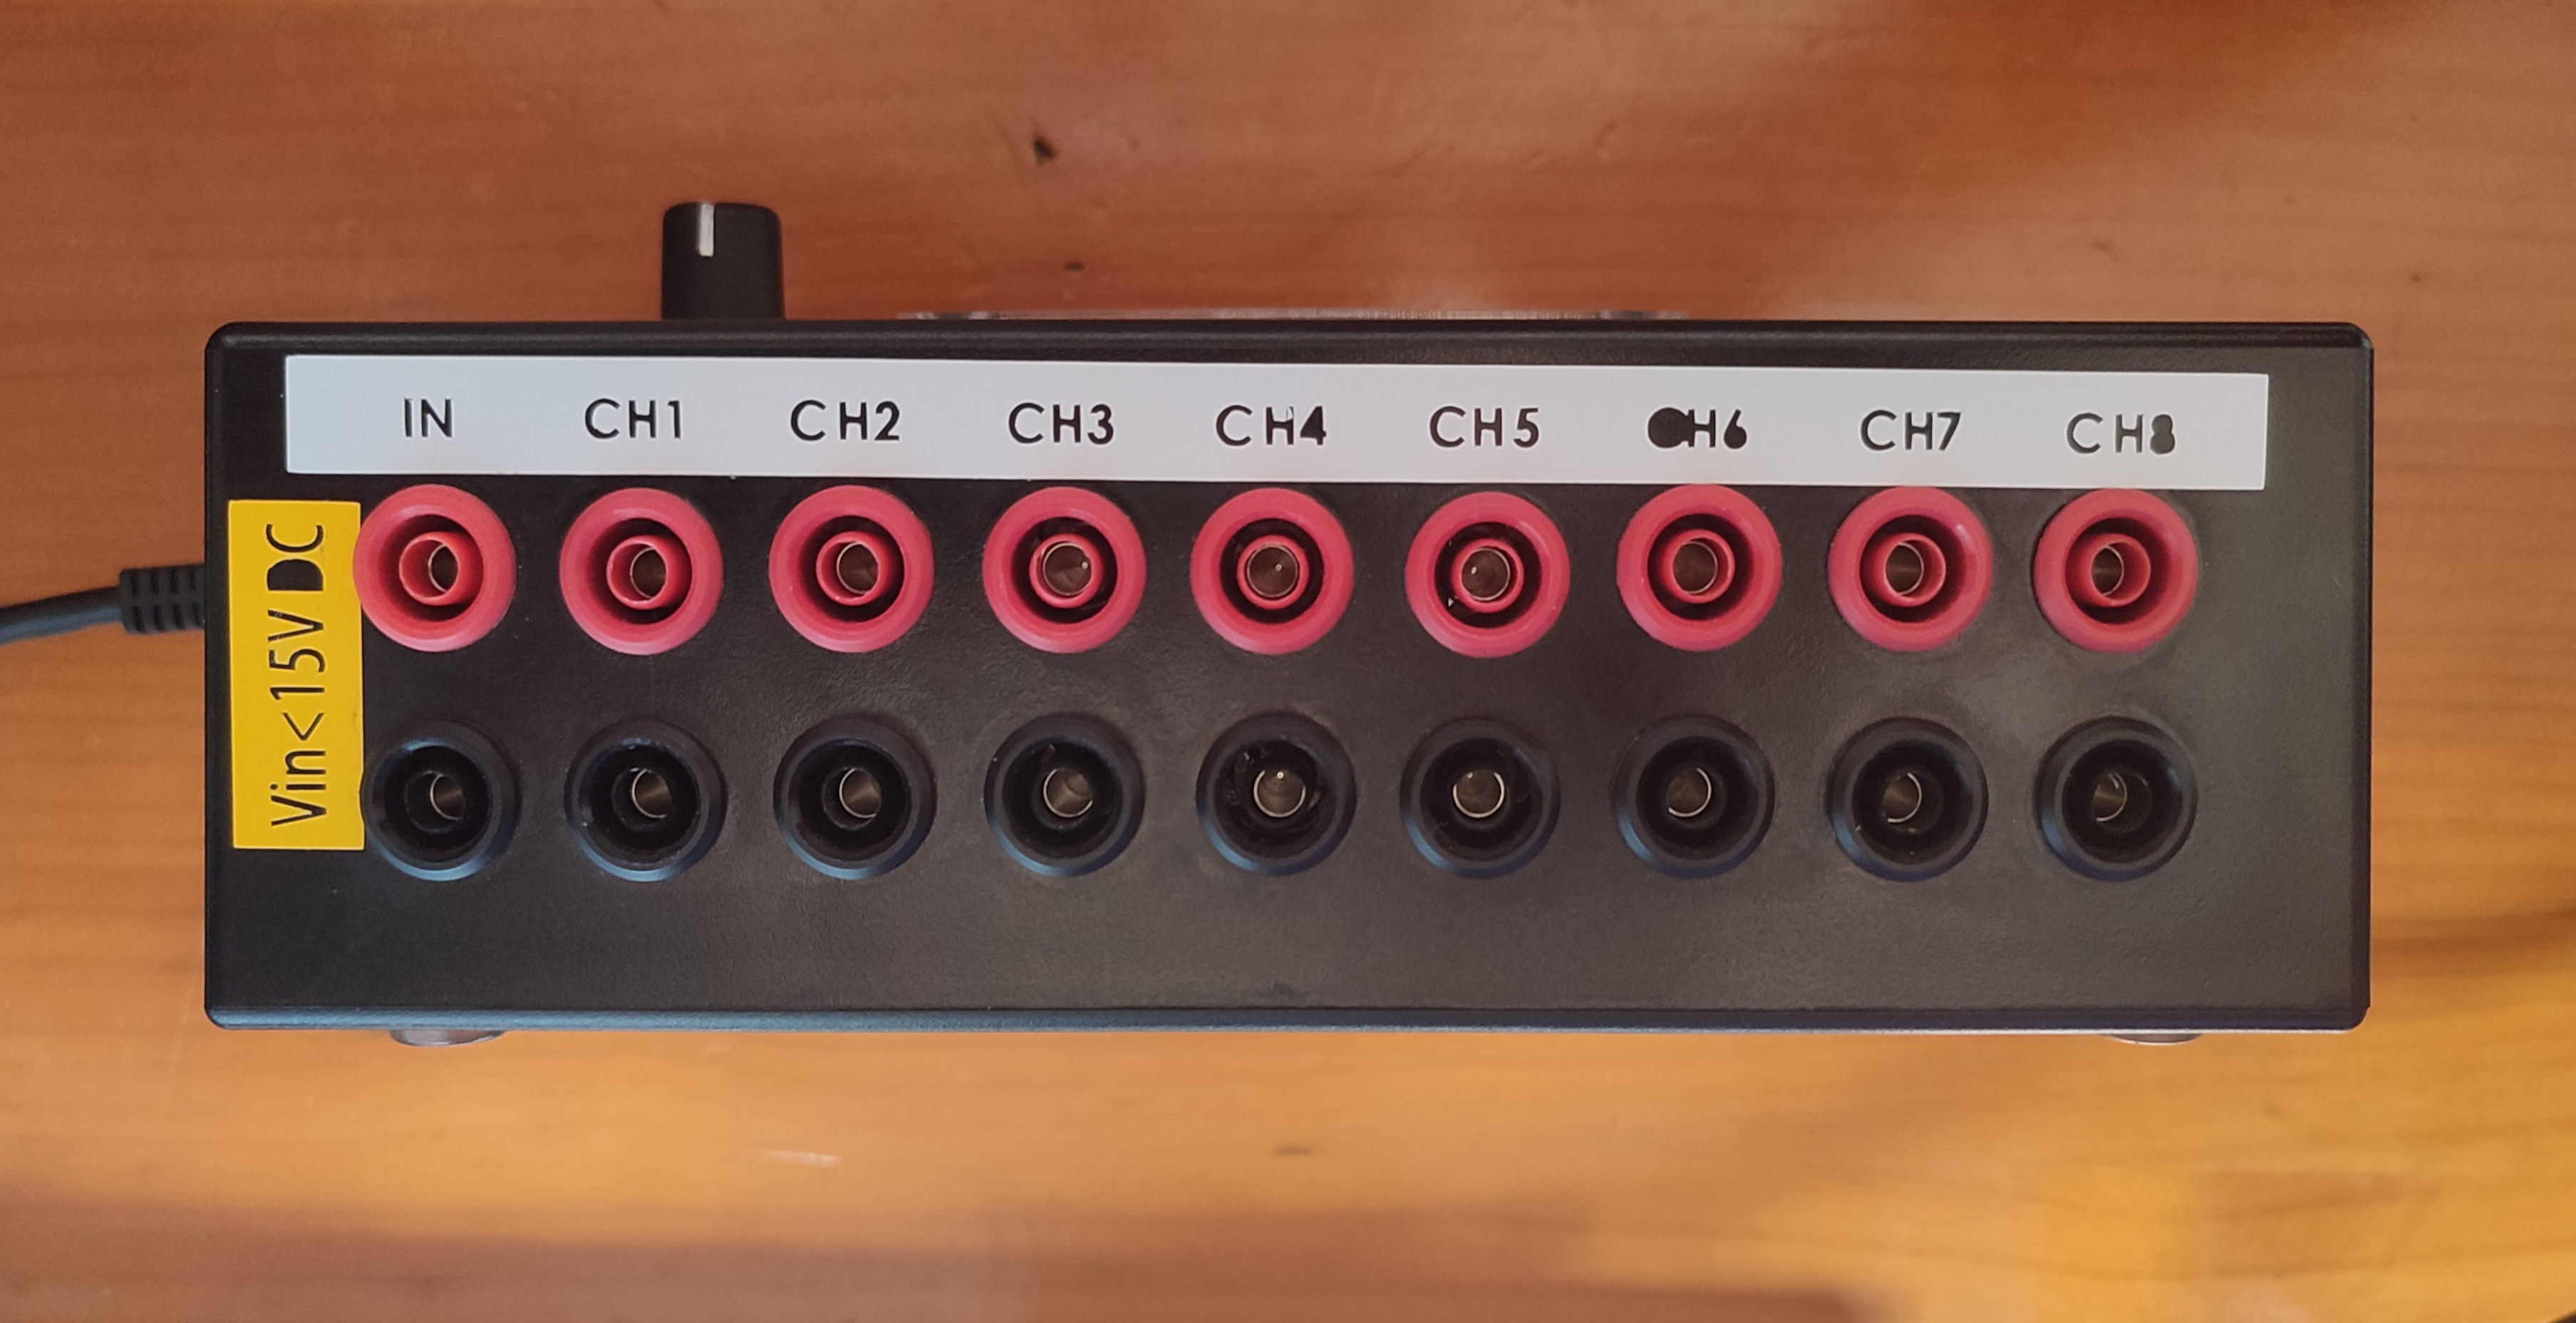
\includegraphics[width=\textwidth]{pwmbox_side.jpg}
    \caption{Lateral del dispositivo PWM Box.}
    \label{fig:pwmbox_side}
\end{figure}


\section{Conocimientos previos}
\label{sec:conocimientos}

En la realización de este trabajo se han puesto en práctica competencias adquiridas en distintas asigntauras de la titulación, y más concretamente de la rama que he cursado, \emph{Ingeniería de Computadores}. Por nombrar algunas:

\begin{itemize}
    \item\textbf{Fundamentos y Metodología de la Programación:} Tratándose de un trabajo de desarrollo, se deben mencionar las asignaturas del Grado en las que se establecen los pilares del conocimiento en programación de muchos estudiantes. Desde lo más básico hasta conceptos más complejos, una gran parte de su contenido se ha aplicado en el desarrollo de este TFG.
    \item\textbf{Estructuras de Datos:} Como su nombre indica, se centra en los distintos contenedores de datos (vectores, colas, pilas, etc), sus particularidades, y cómo trabajar con ellos, conocimientos que han sido de gran utilidad a lo largo de este proyecto.
    \item\textbf{Sistemas con Microprocesadores:} Esta asignatura sirve de introducción a numerosos aspectos de la programación de microcontroladores, culminando en la construcción de un robot de lucha usando un Arduino. Todo ello ha sido puesto en práctica para desarrollar el firmware expuesto.
    \item\textbf{Sistemas Empotrados:} Complementa a la anterior, entrando más en detalle en la arquitectura de los microcontroladores, y aún a más bajo nivel. Aporta conocimientos que han sido de gran valor a lo largo de este proyecto.
    % \item\textbf{Informática Gráfica:} En un principio la relación puede ser menos clara que en los casos anteriores, pero en ella construí una aplicación para visualizar modelos en 3D, un proyecto bastante similar a una parte de las tareas realizadas en este caso.
\end{itemize}

\section{Objetivos}
\label{sec:objetivos}

El objetivo general de este TFG es mejorar el firmware de la versión existente del dispositivo, al que llamaremos \emph{PWM Box}, corrigiendo algunos errores presentes en ella y añadiendo nuevas funcionalidades. Además, se plantea la implementación de una interfaz gráfica compatible con Windows y Linux, que permita el almacenamiento y gestión de distintos perfiles de configuración para el dispositivo.

A raíz de este, se han concretado otros objetivos más definidos:

\begin{itemize}
    \item\textbf{Ingeniería inversa de la versión actual:} Análisis en profundidad el estado actual del dispositivo, entendiendo su funcionamiento e identificando posibles mejoras a implementar.
    \item\textbf{Almacenamiento de perfiles en el microcontrolador:} Utilización de la memoria EEPROM del microcontrolador para almecenar datos que convenga mantener de forma no volátil.
    \item\textbf{Funcionalidad compatible con faros de baja velocidad:} Implementación de un nuevo modo de funcionamiento que permita también probar faros de baja velocidad, es decir, que requieran señales de una frecuencia inferior a las que el dispositivo está programado para producir.
    \item\textbf{Interfaz gráfica:} Diseño de una aplicación para ordenador que permita gestionar la configuración del dispositivo tanto desde Windows como desde Linux. Esta ha de ser capaz de obtener las configuraciones almacenadas en el PWM Box, guardarlas de forma permanente en el disco, y posteriormente volver a cargarlas en el dispositivo.
\end{itemize}

\section{Estructura del documento}

Este documento se divide en distintos apartados, centrándose cada uno en un aspecto distinto del tema que trata:

\begin{itemize}
    \item\textbf{Introdución:} El primer apartado, en el cual nos encontramos, sirve de introducción al proyecto. Proporciona información general del desarrollo que se va a abordar, proporcionando contexto y definiendo a grandes rasgos algunos de las tareas que se van a llevar a cabo.
    \item\textbf{Estado del arte:} En segundo lugar, se realizará un análisis del estado del proyecto antes de empezar a trabajar en él. Se tratará de describir de forma detallada las características de las versiones anteriores del firmware, identificando áreas en las que mejorar y comenzando a tomar algunas decisiones de cara al diseño de la aplicación.
    \item\textbf{Tecnologías:} En este apartado se hará una comparativa de las diferentes tecnologías y herramientas que se han planteado usar en el transcurso del desarrollo, detallando brevemente las motivación de cada una de las elecciones tomadas.
    \item\textbf{Diseño y desarrollo:} Esta parte se centrará en el proceso de ideación y posterior creación de la solución final, explicando paso a paso distintos aspectos de interés del desarrollo.
\end{itemize}

